% RESULTADOS-------------------------------------------------------------------

\chapter{ANÁLISE E RESULTADOS}
\label{chap:resultados}

Este capítulo tem o propósito de demonstrar e fazer a análise dos resultados obtidos no trabalho.
Serão analisados os seguintes resultados:

\begin{itemize}
    \vspace{0.5em}
    \item Reconstrução dos cenários virtuais;
    \item Reconstrução dos cenários reais;
    \item Resultados dos contextos virtuais;
    \item Resultados dos contextos reais;
    \item Desempenho dos algoritmos de cálculo de volume e superfície.
    \item Comparação entre reconstrução em simulação e no experimento;
\end{itemize}
\vspace{1em}

Os resultados da reconstrução de ambas coletas serão avaliados de duas formas: a primeira será a avaliação individual de cada cenário, enquanto que a segunda será a avaliação dos contextos.
Além de fazer a análise da simulação separada da análise em campo, serão comparados os resultados obtidos nos cenários e contextos virtuais com os reais.
Outra análise que será realizada é em relação ao desempenho dos algoritmos de cálculo de volume e superfície, pois esses influenciam diretamente na taxa de acerto da reconstrução.


\section{Simulação virtual}

\subsection{Avaliação da reconstrução dos cenários}
\label{sec:avaliacao_cenarios_simulacao}

Os resultados da reconstrução dos cenários, apresentados na Seção \ref{sec:simulation}, estão retratados na Tabela  \ref{tab:tabela_result_cenarios_sup}, na Tabela \ref{tab:tabela_result_cenarios_vol} e na Figura \ref{fig:recontrucao_virtual}.
A Tabela \ref{tab:tabela_result_cenarios_sup} mostra o resultado da reconstrução da superfície através da diferença entre a área esperada e a área calculada pelo algoritmo.
A avaliação do desempenho da reconstrução em 3D é ditada pela taxa de acerto destes dados.

A superfície foi maior do que o esperado nos cenários A e B porque os pontos da nuvem não ficarão alinhados em um único plano e isso faz com que a triangulação fique desparelha, como se a parede reconstruída parecesse "amassada".
No cenário C o resultado foi menor do que o esperado, pois na coleta quando o robô estava se aproximando ao solo, os sinais com maior intensidade estavam vindo do solo e não da rampa, problema causado pela ambiguidade (Seção \ref{sec:imagem_acustica}).
Além disso, o cenário C possui apenas 22 uc de profundidade, enquanto que o esperado era de 30 uc.

\begin{table}[H]
    \centering
    \caption{Resultados obtidos do cálculo de superfície de cada cenário.}
    \begin{tabular}{@{}ccccc@{}}
        \toprule
        \textbf{Cenário} & \textbf{Superfície esperada} & \textbf{Superfície calculada} & \textbf{Diferença} & \textbf{Taxa de acerto} \\ \midrule
        \textbf{A} & 1.200,00 uc$^2$ & 1.273,57 uc$^2$ & 73,57 uc$^2$ & 93,87\% \\
        \textbf{B} & 1.200,00 uc$^2$ & 1.280,02 uc$^2$ & 80,02 uc$^2$ & 93,33\% \\
        \textbf{C} & 1.697,06 uc$^2$ & 1.591,02 uc$^2$ & 106,04 uc$^2$ & 93,75\% \\ \bottomrule
    \end{tabular}
    \label{tab:tabela_result_cenarios_sup}
\end{table}

A Tabela \ref{tab:tabela_result_cenarios_vol} mostra os resultados de cada cenário em relação ao volume.
Os resultados do cálculo de volume não são diferentes em relação ao cálculo de superfície, portantos os motivos são os mesmos.

A Figura \ref{fig:recontrucao_virtual} mostra o processo de reconstrução dos três cenários. 
A primeira imagem mostra a criação da nuvem de pontos após a etapa de pré-processamento.
A segunda imagem mostra a nuvem de pontos após a etapa de filtragem.
Na terceira imagem, a reconstrução da superfície.
A última imagem exibe o volume gerado a partir da superfície.

\begin{table}[H]
    \centering
    \caption{Resultados obtidos do cálculo de volume de cada cenário.}
    \begin{tabular}{@{}ccccc@{}}
        \toprule
        \textbf{Cenário} & \textbf{Volume esperado} & \textbf{Volume calculado} & \textbf{Diferença} & \textbf{Taxa de acerto} \\ \midrule
        \textbf{A} & 36.000,00 uc$^3$ & 37.862,51 uc$^3$ & 1.862,51 uc$^3$ & 94,83\% \\
        \textbf{B} & 1.200,00 uc$^3$ & 1.251,83 uc$^3$ & 51,83 uc$^3$ & 95,68\% \\
        \textbf{C} & 18.000,00 uc$^3$ & 16.830.45 uc$^3$ & 1.169,54 uc$^3$ & 93,50\% \\ \bottomrule
    \end{tabular}
    \label{tab:tabela_result_cenarios_vol}
\end{table}

\begin{figure}[H]
    \centering
    \caption{Reconstrução dos cenários em simulação virtual.}
    \label{fig:recontrucao_virtual}
    \begin{subfigure}[t]{\textwidth}
        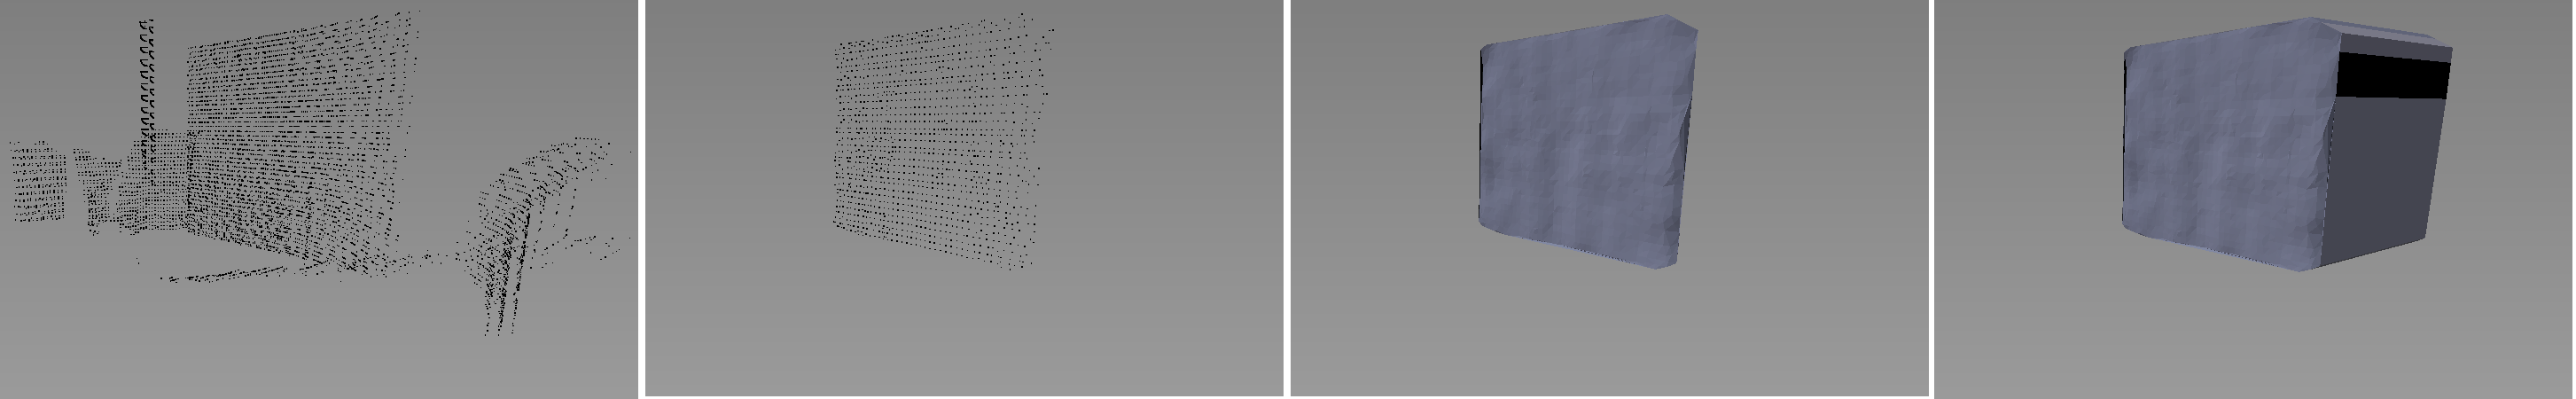
\includegraphics[width=\textwidth]{dados/figuras/wall3.png}
        \caption{Cenário A}
    \end{subfigure}
    \begin{subfigure}[t]{\textwidth}
        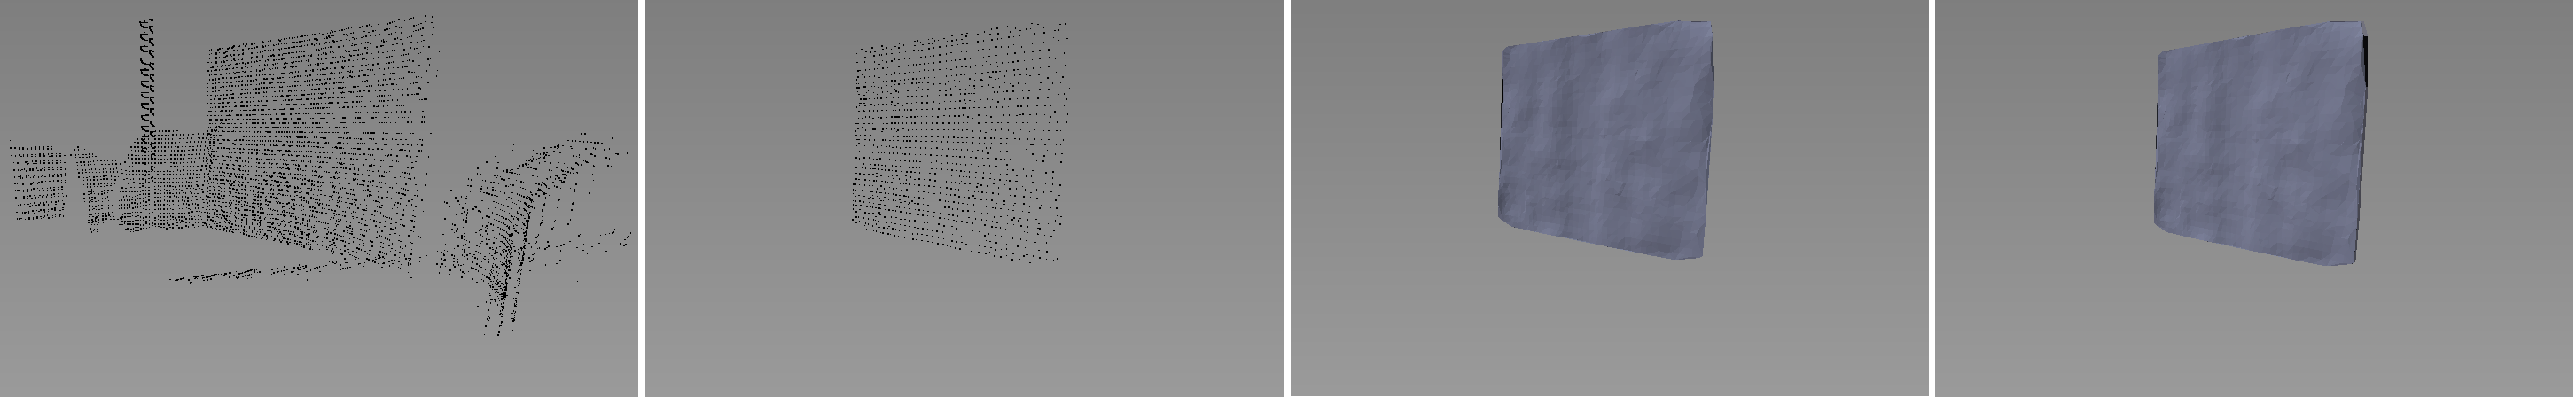
\includegraphics[width=\textwidth]{dados/figuras/wall.png}
        \caption{Cenário B}
    \end{subfigure}
    \begin{subfigure}[t]{\textwidth}
        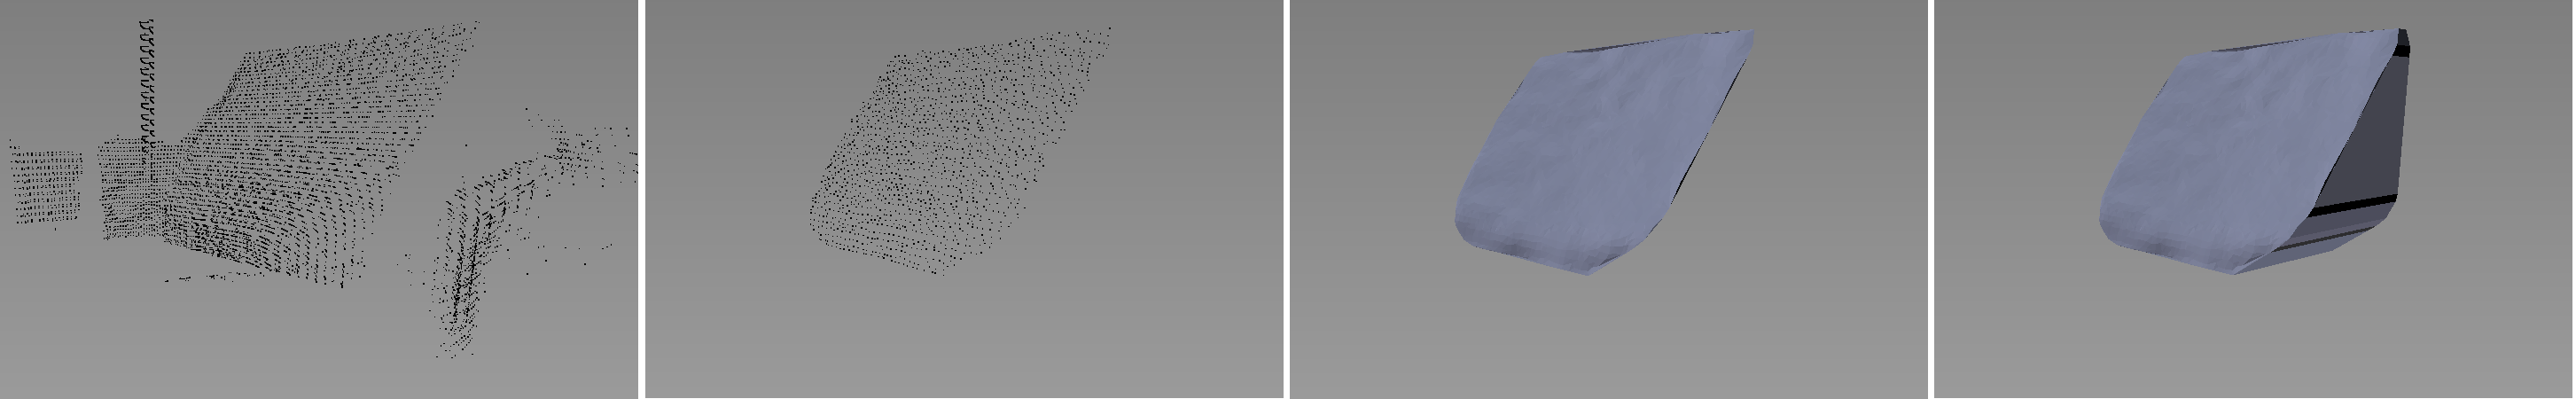
\includegraphics[width=\textwidth]{dados/figuras/declined.png}
        \caption{Cenário C}
    \end{subfigure}
\end{figure}

\subsection{Avaliação dos contextos}
\label{sec:avaliacao_contextos}

Essa seção descreve os resultados obtidos nas comparações de cenários, os chamados contextos (os contextos foram descritos na Seção \ref{sec:simulation}).

No primeiro contexto (AB), o volume calculado foi quase igual ao esperado, porém não foi melhor por causa de pequenos ruídos remanescentes e da própria reconstrução afetar levemente de forma negativa na taxa de acerto.
O segundo contexto (AC) foi obtido um resultado abaixo em relação ao contexto anterior.
O principal motivo foi por conta da determinação do plano base, em outras palavras, a distância entre o plano base e a malha no cenário A é de 30 uc, enquanto que no contexto AC o plano base está a 22 uc.
Resultando em um volume menor, diminuindo o valor da diferença de volume do contexto.
Os resultados dos contexto estão descritos na Tabela \ref{tab:tabela_resultados_contextos_sim} e os volumes reconstruídos estão exibidos na Figura \ref{fig:recontrucao_virtual}.

\begin{table}[H]
    \centering
    \caption{Resultados obtidos do cálculo de comparação de volume dos contextos em simulação.}
    \begin{tabular}{ccccc}
        \toprule
        \textbf{Contexto} & \textbf{Volume esperado} & \textbf{Volume calculado} & \textbf{Diferença} & \textbf{Taxa de acerto} \\ \midrule
        \textbf{AB} & 6.000 uc$^3$ & 6.288,77 uc$^3$ & 288,77 uc$^3$ & 95,41\% \\
        \textbf{AC} & 18.000 uc$^3$ & 11.594,48 uc$^3$ & 6.405,52 uc$^3$ & 64,41\% \\ \bottomrule
    \end{tabular}
    \label{tab:tabela_resultados_contextos_sim}
\end{table}

\begin{figure}[H]
    \centering
    \caption{Reconstrução dos cenários nos contextos.}
    \label{fig:recontrucao_virtual}
    \begin{subfigure}[t]{0.33\textwidth}
        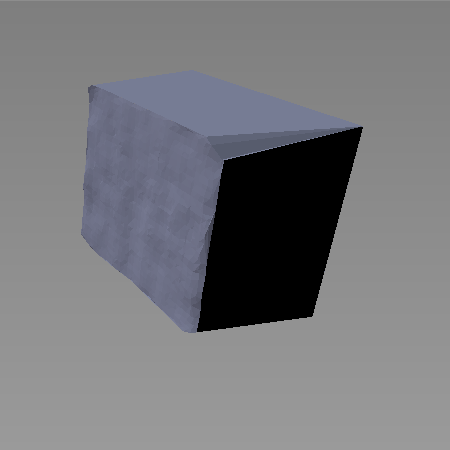
\includegraphics[width=\textwidth]{dados/figuras/AC1.png}
        \caption{Cenário A no contexto AB.}
    \end{subfigure}
    \hspace{1em}
    \begin{subfigure}[t]{0.33\textwidth}
        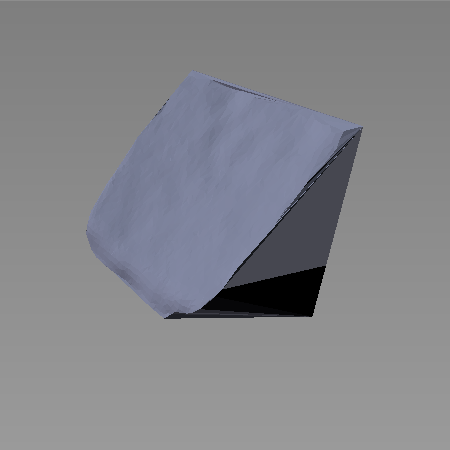
\includegraphics[width=\textwidth]{dados/figuras/AC2.png}
        \caption{Cenário B no contexto AB.}
    \end{subfigure}
    \begin{subfigure}[t]{0.33\textwidth}
        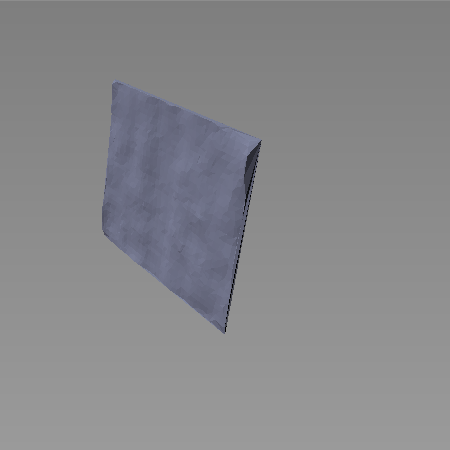
\includegraphics[width=\textwidth]{dados/figuras/AB1.png}
        \caption{Cenário A no contexto AC.}
    \end{subfigure}
    \hspace{1em}
    \begin{subfigure}[t]{0.33\textwidth}
        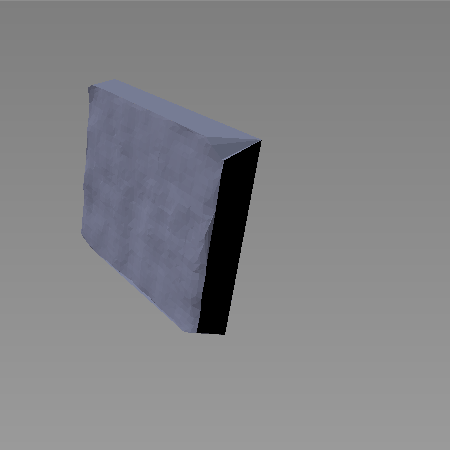
\includegraphics[width=\textwidth]{dados/figuras/AB2.png}
        \caption{Cenário C no contexto AC.}
    \end{subfigure}
\end{figure}


\section{In loco}

\subsection{Avaliação da reconstrução do cenário}
\label{sec:avaliacao_cenarios_inloco}
Nesta seção, serão descritos os resultados obtidos na comparação realizada \textit{in loco}, no qual os cenários estão descritos na Seção \ref{sec:in_loco}.
Diferente da simulação, a unidade de medida utilizada no experimento é o metro.
A parede analisada da piscina, possui 1,18m de altura (contando apenas a parte submersa) e 2,1m de largura.
Como descrito anteriormente, são dois os cenários estudados: no cenário D o ROV está a 1,5m de distância da parede, enquanto que no cenário E, está a 3m.

A primeira análise do experimento será a área de superfície, onde o resultado esperado é de 2,478m$^2$\footnote{Considerando a parede reta.}.
A variação vertical nos dados coletados é de 0,7m por causa do corpo do ROV, que ocupa 0,4m, impedindo que o sensor prossiga até o fundo da piscina (o sensor fica acoplado na parte superior do robô).
Portanto o robô realizou o escaneamento de 0,7m apesar da parede possuir 1,18m de altura. 

A Tabela \ref{tab:result_inloco_sup} mostra a superfície esperada levando em consideração ambos os casos (a altura total e a altura percorrida pelo sensor).
Analisando o cenário D e levando em consideração a altura total (1,18m), o resultado do foi menor do que o esperado pelo simples motivo que o robô percorreu apenas 0,7m da altura.
Levando em consideração a altura percorrida (0,7m), o resultado foi maior do que o esperado por conta da parede reconstruída ser curvada, enquanto que a superfície esperada não leva esse detalhe em conta.
O cenário E apresentou resultados semelhantes ao cenário anterior.

\begin{table}[H]
    \centering
    \caption{Resultados obtidos do cálculo de superfície, levando em conta a variação de altura na coleta.}
    \begin{tabular}{@{}ccccc@{}}
        \toprule
        \multicolumn{1}{c}{\textbf{Cenário}} & \textbf{Superfície esperada} & \textbf{Superfície calculada} & \textbf{Diferença} & \textbf{Taxa de acerto} \\ \midrule
        \textbf{D (0,70m)} & 1,51m$^2$ & 1,96m$^2$ & 0,45m$^2$ & 77,04\% \\
        \textbf{D (1,18m)} & 2,48m$^2$ & 1,96m$^2$ & 0,52m$^2$ & 79,03\% \\
        \textbf{E (0,70m)} & 1,51m$^2$ & 1,92m$^2$ & 0,41m$^2$ & 78,64\% \\
        \textbf{E (1,18m)} & 2,48m$^2$ & 1,92m$^2$ & 0,56m$^2$ & 77,42\% \\
        \bottomrule
    \end{tabular}
    \label{tab:result_inloco_sup}
\end{table}

\subsection{Avaliação do contexto}

A avaliação do cálculo de volume do contexto DE vai seguir o mesmo padrão da avaliação do cálculo de área de superfície de ambos cenários envolvidos nesse contexto.
Portanto, haverá o contexto onde é considerado apenas a altura escaneada pelo sensor (0,7m) e outro onde o contexto considera toda a altura da parede (1,18m).

\begin{table}[H]
    \centering
    \caption{Resultados obtidos da comparação de volume no contexto em campo.}
    \begin{tabular}{@{}ccccc@{}}
        \toprule
        \textbf{Contexto} & \textbf{Volume esperado} & \textbf{Volume calculado} & \textbf{Diferença} & \textbf{Taxa de acerto} \\ \midrule
        \textbf{DE (0,70m)} & 2,20m$^3$ & 2,06m$^3$ & 0,14m$^3$ & 93,64\% \\
        \textbf{DE (1,18m)} & 3,72m$^3$ & 2,06m$^3$ & 1,66m$^3$ & 55,38\% \\ \bottomrule
    \end{tabular}
    \label{tab:result_inloco_vol}
\end{table}